\documentclass[a4paper, 10pt]{article}
\usepackage{CEDT-Homework-style}

\usepackage{amsmath}
\allowdisplaybreaks

\setlength{\headheight}{14.49998pt}

\begin{document}
\subject[2110205 - Statistics for Computer Engineering]
\hwtitle{2}{Week 1 - 2}{6733172621 Patthadon Phengpinij}{ChatGPT (for LaTeX styling and grammar checking)}


% ================================================================================ %
\section{Week 1: Counting and Probability}
% ================================================================================ %



% ================================================================================ %
%                                    Problem 01                                    %
% ================================================================================ %
\begin{problem}
Consider the following Python code.
\begin{codingbox}
s = 1
for i in range(1, n):
    s = s * i
for i in range(1, n-k):
    s = s / k
print(s)
\end{codingbox}
What does this code compute?
\end{problem}

\begin{solution}
From the first for loop, \( i \) equals \( 1,\, 2,\, 3,\, ...,\, n-1 \),
which means \( s \) equals \( (n-1)! \). \par

The Second loop makes \( i \) equals \( 1,\, 2,\, 3,\, ...,\, n-k-1 \),
which means \( s \) equals \( \cfrac{(n-1)!}{(n-k-1)!} \). \par

Therefore, when this program finished running, s equals
\begin{align*}
    \cfrac{(n-1)!}{(n-k-1)!} &= \cfrac{(n-1)!}{\paren{(n-1) - k}!} \\
    &= \boxed{\text{b.)}\;_{n-1}P_k}
\end{align*}
\end{solution}
% ================================================================================ %


% ================================================================================ %
%                                    Problem 02                                    %
% ================================================================================ %
\begin{problem}
In a class, 60 students can play piano, 40 students can play the violin,
20 students can play both, and 50 students can play neither.
How many students are there in the class?
\end{problem}

\begin{solution}
\par
\begin{center}
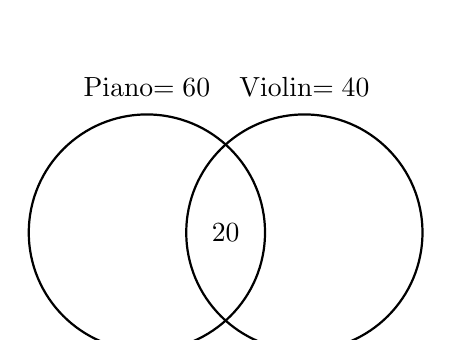
\begin{tikzpicture}
    % Draw circles
    \draw[thick] (0,0) circle (1.5cm) node[above=1.6cm] {Piano\( = 60 \)};
    \draw[thick] (2,0) circle (1.5cm) node[above=1.6cm] {Violin\( = 40 \)};

    % Labels inside
    \node at (1.0,0) {20};
\end{tikzpicture}
\end{center}

\par From the diagram, we can see that
the number of students who can play only the piano is \( 60 - 20 = 40 \),
the number of students who can play only the violin is \( 40 - 20 = 20 \).
\\
\par Therefore, the total number of students in the class is:
\begin{align*}
    40 + 20 + 20 + 50 = \boxed{130}
\end{align*}
\end{solution}
% ================================================================================ %


% ================================================================================ %
%                                    Problem 03                                    %
% ================================================================================ %
\begin{problem}
There are 10 people in a committee.
How many ways can they select the president, vice president, secretary, and treasurer,
given that one person can hold at most one position?
\end{problem}

\begin{solution}
We can say that,
\begin{enumerate}[wide=0pt, itemsep=2pt, parsep=0pt, leftmargin=*]
    \item The first position can be filled by any of the 10 people.
    \item The second position can be filled by any of the remaining 9 people.
    \item The third position can be filled by any of the remaining 8 people.
    \item The fourth position can be filled by any of the remaining 7 people.
\end{enumerate}

Therefore, the total number of ways to select the four positions is:
\begin{align*}
    10 \times 9 \times 8 \times 7 = \boxed{5040}
\end{align*}
\end{solution}
% ================================================================================ %


% ================================================================================ %
%                                    Problem 04                                    %
% ================================================================================ %
\begin{problem}
There are 8 men and 6 women in a class.
How many ways can the professor select 3 men and 3 women to attend a conference?
\end{problem}

\begin{solution}
We can say that,
\begin{enumerate}[wide=0pt, itemsep=2pt, parsep=0pt, leftmargin=*]
    \item The number of ways to select 3 men from 8 is given by \(\binom{8}{3}\).
    \item The number of ways to select 3 women from 6 is given by \(\binom{6}{3}\).
\end{enumerate}

Therefore, the total number of ways to select 3 men and 3 women is:
\begin{align*}
    \binom{8}{3} \times \binom{6}{3} &= \frac{8!}{3!(8-3)!} \times \frac{6!}{3!(6-3)!} \\
    &= \frac{8!}{3!5!} \times \frac{6!}{3!3!} \\
    &= \frac{8 \times 7 \times 6}{3 \times 2 \times 1} \times \frac{6 \times 5 \times 4}{3 \times 2 \times 1} \\
    &= \frac{336}{6} \times \frac{120}{6} \\
    &= 56 \times 20 \\
    &= \boxed{1120}
\end{align*}
\end{solution}
% ================================================================================ %


% ================================================================================ %
%                                    Problem 05                                    %
% ================================================================================ %
\begin{problem}
For an arbitrary day in August, there is probability 0.4 that it is rainy, and 0.35 that it is windy.
Also, there is probability 0.25 that it is rainy but \textbf{not} windy.
What is the probability that the day is neither rainy nor windy?
\end{problem}

\begin{solution}
Let \( R \) be the event that it is rainy and \( W \) be the event that it is windy. \\
Thus, \( P(R) = 0.40, \; P(W) = 0.35, \; P(R \cap W') = 0.25 \).

We want to find the probability that the day is neither rainy nor windy, which is given by:
\begin{align*}
    P(R' \cap W') &= 1 - P(R \cup W) \\
    &= 1 - (P(W) + P(R \cap W')) \\
    &= 1 - (0.35 + 0.25) \\
    &= 1 - 0.60 \\
    &= 0.40
\end{align*}

Therefore, the probability that the day is neither rainy nor windy is \( \boxed{0.40} \).
\end{solution}
% ================================================================================ %


% ================================================================================ %
%                                    Problem 06                                    %
% ================================================================================ %
\begin{problem}
Benz rolls two dice.
What is the probability that the difference of the numbers on both dice is \textbf{at most 3}?
\end{problem}

\begin{solution}
To find the probability that the difference of the numbers on both dice is at most 3,
we can first determine the total number of outcomes when rolling two dice.
\\
\par Since each die has 6 faces, the total number of outcomes is \( 6 \times 6 = 36 \).
\\
\par Next, we need to count the number of favorable outcomes where the absolute difference between the two dice is at most 3.
We can list the possible outcomes for each pair of rolls:
\begin{enumerate}
    \item If the first die shows 1, the second die can show: 1, 2, 3, 4 (4 outcomes)
    \item If the first die shows 2, the second die can show: 1, 2, 3, 4, 5 (5 outcomes)
    \item If the first die shows 3, the second die can show: 1, 2, 3, 4, 5, 6 (6 outcomes)
    \item If the first die shows 4, the second die can show: 1, 2, 3, 4, 5, 6 (6 outcomes)
    \item If the first die shows 5, the second die can show: 2, 3, 4, 5, 6 (5 outcomes)
    \item If the first die shows 6, the second die can show: 3, 4, 5, 6 (4 outcomes)
\end{enumerate}

Now, we can sum these favorable outcomes: \( 4 + 5 + 6 + 6 + 5 + 4 = 30 \)

Thus, the probability that the difference of the numbers on both dice is at most 3 is:
\[
P(\text{difference} \leq 3) = \frac{30}{36} = \frac{5}{6}
\]

Therefore, the final answer is \( \boxed{\frac{5}{6}} \)
\end{solution}
% ================================================================================ %


% ================================================================================ %
%                                    Problem 07                                    %
% ================================================================================ %
\begin{problem}
Jam tosses a coin 6 times.
What is the probability that it will land head 3 times and tail 3 times?
\end{problem}

\begin{solution}
Each toss of the coin is independent, and the probability of getting head or tail is \( \frac{1}{2} \).
\\
\par The number of ways to choose 3 heads (and thus 3 tails) in 6 tosses is given by the binomial coefficient:
\[
\binom{6}{3} = \frac{6!}{3!3!} = 20
\]
\\
\par Therefore, the probability of getting exactly 3 heads and 3 tails is:
\[
P(\text{3 heads, 3 tails}) = \binom{6}{3} \left( \frac{1}{2} \right)^6 = 20 \times \frac{1}{64} = \frac{20}{64} = \boxed{\frac{5}{16}}
\]
\end{solution}
% ================================================================================ %


\pagebreak


% ================================================================================ %
%                                    Problem 08                                    %
% ================================================================================ %
\begin{problem}
A mobile game has a gacha (loot box) with a 10\% chance of getting a rare character.
Non pulls the gacha 4 times. What is the probability that she gets \textbf{at least} one rare character?
\end{problem}

\begin{solution}
To find the probability of getting at least one rare character in 4 pulls, we can use the complement rule.
First, we calculate the probability of not getting a rare character in a single pull, which is \(1 - 0.1 = 0.9\).

The probability of not getting a rare character in all 4 pulls is:
\[
P(\text{no rare character in 4 pulls}) = (0.9)^4 = 0.6561
\]

Therefore, the probability of getting at least one rare character in 4 pulls is:
\begin{align*}
    P(\text{at least 1 rare character in 4 pulls}) &= 1 - P(\text{no rare character in 4 pulls}) \\
    &= 1 - 0.6561 \\
    &= \boxed{0.3439}
\end{align*}
\end{solution}
% ================================================================================ %


% ================================================================================ %
%                                    Problem 09                                    %
% ================================================================================ %
\begin{problem}
In a horse racing with 8 horses, a player guesses which horses will finish first
and second (assuming that every permutation of finishing occurs with equal probability).
The player wins if he guesses \textbf{at least} one position correctly.
\begin{subproblems}
    \item If a player guesses two different horses in both positions, what is his probability of winning?
    \item If a player guesses the same horse in both positions, what is his probability of winning?
    \item From a), and b), what is the best strategy for winning?
\end{subproblems}
\end{problem}

\begin{solution}
\par\noindent\textbf{a).} If a player guesses two different horses in both positions,
each position would have the probability of winning equal to \( \frac{1}{8} \),
since there are 8 horses to choose from and the choices are independent.
\\
\par The total number of possible outcomes (permutations of 8 horses taken 2 at a time) is:
\[
8 \times 7 = 56
\]
Thus, the probability of winning by guessing both first and second place correctly is \( \frac{1}{56} \)
So that, the probability of winning in this case is:
\begin{align*}
    P(\text{winning}) &= \frac{1}{8} + \frac{1}{8} - \frac{1}{56} \\
    &= \frac{7}{56} + \frac{7}{56} - \frac{1}{56} \\
    &= \boxed{\frac{13}{56}}
\end{align*}

\par\noindent\textbf{b).} If a player guesses the same horse in both positions,
since that horse can be in any position (from \(8\) positions),
there are \(2\) out of \(8\) choices for the horse he guessed to win.
\[
P(\text{winning}) = \frac{2}{8} = \boxed{\frac{1}{4}}
\]

\par\noindent\textbf{c).} From a), and b), the best strategy for winning is:
\[
\boxed{\text{to guess the \textbf{same horse in both positions}}},
\]
as this gives a probability of winning of \(\frac{1}{4}\) (which equal to \(\frac{14}{56}\)),
compared to only \(\frac{13}{56}\) when guessing two different horses.
\end{solution}
% ================================================================================ %


% ================================================================================ %
%                                    Problem 10                                    %
% ================================================================================ %
\begin{problem}
Mint tosses 8 coins. If it is known that the number of heads is at most 2,
what is the probability that there are exactly 2 heads?
\end{problem}

\begin{solution}
Given, \\
\(A\) := events where there are exactly 2 heads \\
\(B\) := events where there are at most 2 heads \\
We want to find \(P(A|B)\), the probability of \(A\) given \(B\).
\\
\par Using Bayes' theorem:
\[
P(A|B) = \frac{P(A \cap B)}{P(B)}
\]
Since \(A\) is a subset of \(B\), we have \(P(A \cap B) = P(A)\).
\\
\par\textbf{Calculating \(P(A)\)}: \\
The total number of outcomes when tossing 8 coins is \(2^8 = 256\).
The number of favorable outcomes for getting exactly 2 heads (and 6 tails) is given by the binomial coefficient:
\[
P(A) = \frac{\binom{8}{2}}{2^8} = \frac{28}{256} = \frac{7}{64}
\]

\par\textbf{Calculating \(P(B)\)}: \\
The number of favorable outcomes for getting at most 2 heads is the sum of the outcomes for 0, 1, and 2 heads:
\[
P(B) = \frac{\binom{8}{0} + \binom{8}{1} + \binom{8}{2}}{2^8} = \frac{1 + 8 + 28}{256} = \frac{37}{256}
\]

\par Thus,
\[
P(A|B) = \frac{P(A \cap B)}{P(B)} = \frac{P(A)}{P(B)} = \frac{\frac{7}{64}}{\frac{37}{256}} = \frac{7 \times 256}{64 \times 37} = \frac{28}{37}
\]
Thus, the probability that there are exactly 2 heads given that there are at most 2 heads is:
\[
\boxed{\frac{28}{37}}
\]
\end{solution}
% ================================================================================ %



% ================================================================================ %
\pagebreak
\section{Week 2: Independence, Correlation, and Bayes' Theorem}
% ================================================================================ %



% ================================================================================ %
%                                    Problem 11                                    %
% ================================================================================ %
\begin{problem}
Let \(A\), \(B\), and \(C\) be events with probability greater than 0 and less than 1.
Determine whether the following statements are true or false.
\begin{subproblems}
    \item If \(A\) and \(B\) are disjoint, then \(A'\) and \(B'\) must also be disjoint.
    \item If \(A\) and \(B\) are independent, then \(A'\) and \(B'\) must also be independent.
    \item If \(A\) and \(B\) are independent, and \(B\) and \(C\) are independent, then \(A\) and \(C\) must also be independent.
\end{subproblems}
\end{problem}

\begin{solution}
\par\noindent\textbf{a).} If \(A\) and \(B\) are disjoint, then \(A'\) and \(B'\) must also be disjoint. \(\Rightarrow \boxed{\text{`` FALSE ''}}\)
\begin{center}
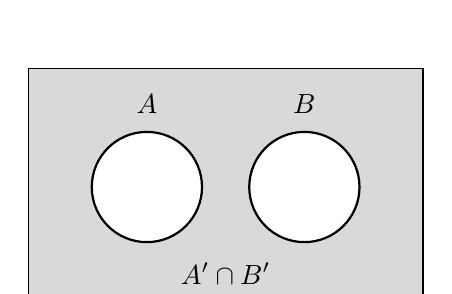
\begin{tikzpicture}
    % Universe rectangle
    \draw[thick] (0,0) rectangle (5,3) node[below left] {\(U\)};

    % Shade intersection of complements (outside both A and B)
    \fill[gray!30] (0,0) rectangle (5,3);

    % Draw set A
    \begin{scope}
        \clip (0,0) rectangle (5,3);
        \fill[white] (1.5,1.5) circle (0.7cm);
        \draw[thick] (1.5,1.5) circle (0.7cm) node[above=0.8cm] {\(A\)};
    \end{scope}

    % Draw set B
    \begin{scope}
        \clip (0,0) rectangle (5,3);
        \fill[white] (3.5,1.5) circle (0.7cm);
        \draw[thick] (3.5,1.5) circle (0.7cm) node[above=0.8cm] {\(B\)};
    \end{scope}

    % Explanation label
    \node at (2.5,0.4) {\(A' \cap B'\)};
\end{tikzpicture}
\end{center}

\par\noindent\textbf{b).} If \(A\) and \(B\) are independent, then \(A'\) and \(B'\) must also be independent.  \(\Rightarrow \boxed{\text{`` TRUE ''}}\)
\proof
\begin{align*}
    P(A' \cap B') &= 1 - P(A \cup B) \\
    &= 1 - (P(A) + P(B) - P(A \cap B)) \\
    &= 1 - (P(A) + P(B) - P(A)P(B)) \\
    &= 1 - P(A) - P(B) + P(A)P(B) \\
    &= \paren{1 - P(A)}\paren{1 - P(B)} \\
    &= P(A')P(B')
\end{align*}

\par\noindent\textbf{c).} If \(A\) and \(B\) are independent, and \(B\) and \(C\) are independent, then \(A\) and \(C\) must also be independent.  \(\Rightarrow \boxed{\text{`` FALSE ''}}\)
\vspace{2mm}
\par\textit{Counterexample.}
Since, \(A\) and \(B\) are independent, and \(B\) and \(C\) are independent. \\
Select \(A = C \; \Rightarrow \; \boxed{A \text{ and } C \text{ are not independent}} \).

\end{solution}
% ================================================================================ %


\pagebreak


% ================================================================================ %
%                                    Problem 12                                    %
% ================================================================================ %
\begin{problem}
Mick tosses a coin 5 times.
Determine whether the two given events are independent or not.
\begin{subproblems}
    \item The event that the first toss is head, and the event that the total number of heads is exactly 3.
    \item The event that the first toss is head, and the event that the total number of heads is an odd number.
\end{subproblems}
\end{problem}

\begin{solution}
\par\noindent\textbf{a).} Given, \\
\( A \) := event where the first toss is head.
\[
    P(A) = \frac{1}{2} \\
\]
\( B \) := event where the total number of heads is exactly 3.
\[
    P(B) = \frac{\binom{5}{3}}{2^5} = \frac{10}{32} \\
\]
\( A \cap B \) := event where the first toss is head and the total number of head of the less 4 tosses is 2.
\[
    P(A \cap B) = \frac{1}{2} \times \frac{\binom{4}{2}}{2^4} = \frac{6}{32} \\
\]
To check for independence, we need to see if \( P(A \cap B) = P(A)P(B) \).
\[
    P(A)P(B) = \frac{1}{2} \times \frac{10}{32} = \frac{5}{32} \\
\]
Since, \( P(A \cap B) = \frac{6}{32} \) and \( P(A)P(B) = \frac{5}{32} \), we have
\[
    P(A \cap B) > P(A)P(B)
\]
Therefore, these two events are \( \boxed{\text{not independent}} \).
\\
\par\noindent\textbf{b).} Given, \\
\( A \) := event where the first toss is head.
\[
    P(A) = \frac{1}{2}
\]
\( B \) := event where the total number of heads is an odd number.
\[
    P(B) = \frac{1}{2}
\]
\( A \cap B \) := event where the first toss is head and the total number of heads is an odd number.
\[
    P(A \cap B) = \frac{1}{2} \times \frac{1}{2} = \frac{1}{4}
\]
To check for independence, we need to see if \( P(A \cap B) = P(A)P(B) \).
\[
    P(A)P(B) = \frac{1}{2} \times \frac{1}{2} = \frac{1}{4}
\]
Since, \( P(A \cap B) = \frac{1}{4} \) and \( P(A)P(B) = \frac{1}{4} \), we have
\[
    P(A \cap B) = P(A)P(B)
\]
Therefore, these two events are \( \boxed{\text{independent}} \).

\end{solution}
% ================================================================================ %


% ================================================================================ %
%                                    Problem 13                                    %
% ================================================================================ %
\begin{tosubmit}
\problem[13]
Moss rolls a die (singular form of dice) 2 times. Determine whether the two given events have positive, zero, or negative correlation.
\begin{subproblems}
    \item The event that first roll is an odd number, and the event that the sum of both rolls is \textbf{at least 9}.
    \item The event that the first roll is prime number, and the event that the sum both rolls is divisible by 4.
    \item The event that the sum of both rolls is an even number, and the event that the sum of both rolls is divisible by 3
\end{subproblems}

\submitsolution
Using the following image of table of sum of two rolls,
\begin{center}
    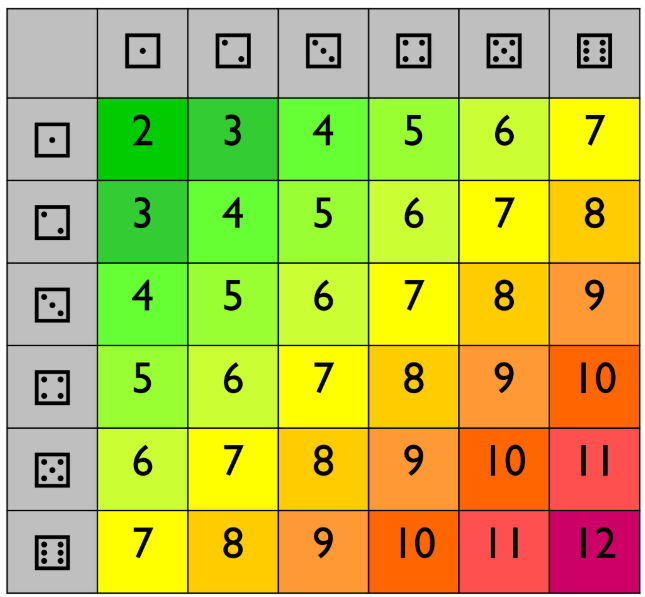
\includegraphics[width=0.25\textwidth]{Images/hw02-dice.png}
\end{center}

\par\noindent\textbf{a).} Given \\
\( A_a \) := events where the first roll is an odd number \\
\( B_a \) := events where the sum of both rolls is at least 9 \\
From the table, we know that,
\begin{center}
    \( P(A_a) = \frac{1}{2},\enspace P(B_a) = \frac{10}{36},\enspace P(A_a \cap B_a) = \frac{4}{36} \)
\end{center}
Consider,
\begin{align*}
    \allowbreak
    P(A_a)P(B_a) &= \frac{1}{2}\times\frac{10}{36} \\
    &= \frac{5}{36} \\
    &> \frac{4}{36} \\
    P(A_a)P(B_a) &> P(A_a \cap B_a)
\end{align*}
Therefore, these two events have \( \boxed{\text{Negative Correlation}} \) \\

\par\noindent\textbf{b).} Given \\
\( A_b \) := events where the first roll is a prime number \\
\( B_b \) := events where the sum of both rolls is divisible by 4 \\
From the table, we know that,
\begin{center}
    \( P(A_b) = \frac{1}{2},\enspace P(B_b) = \frac{9}{36},\enspace P(A_b \cap B_b) = \frac{5}{36} \)
\end{center}
Consider,
\begin{align*}
    \allowbreak
    P(A_b)P(B_b) &= \frac{1}{2}\times\frac{9}{36} \\
    &= \frac{9}{72} \\
    &< \frac{10}{72} \\
    &= \frac{5}{36} \\
    P(A_b)P(B_b) &< P(A_b \cap B_b)
\end{align*}
Therefore, these two events have \( \boxed{\text{Positive Correlation}} \) \\

\par\noindent\textbf{c).} Given \\
\( A_c \) := events where the sum of both rolls is an even number \\
\( B_c \) := events where the sum of both rolls is divisible by 3 \\
From the table, we know that,
\begin{center}
    \( P(A_c) = \frac{18}{36},\enspace P(B_c) = \frac{12}{36},\enspace P(A_c \cap B_c) = \frac{6}{36} \)
\end{center}
Consider,
\begin{align*}
    P(A_c)P(B_c) &= \frac{18}{36}\times\frac{12}{36} \\
    &= \frac{1}{6} \\
    &= \frac{6}{36} \\
    P(A_c)P(B_c) &= P(A_c \cap B_c)
\end{align*}
Therefore, these two events have \( \boxed{\text{Zero Correlation}} \)
\end{tosubmit}
% ================================================================================ %


% ================================================================================ %
%                                    Problem 14                                    %
% ================================================================================ %
\begin{problem}
A mobile game has a gacha (loot box) with a 20\% chance of getting a rare character.
Furthermore, when pulling 5 consecutive rolls, if there is no rare character among the first 4 rolls,
then the 5th roll is guaranteed to be a rare character (otherwise, the 5th roll will just have a normal rate).
Fai pulls the gacha 5 times. What is the probability that her 5th roll is a rare character?
\end{problem}

\begin{solution}
Let \( A \) be the event that Fai's 5th roll is a rare character. \\
We can find \( P(A) \) by considering two cases:
\\
\par\noindent\textbf{Case 1:} There is at least one rare character among the first 4 rolls.
\begin{enumerate}
    \item The probability of this happening is \( 1 - (0.8)^4 = 1 - 0.4096 = 0.5904 \).
    \item If this case occurs, the 5th roll has a 20\% chance of being a rare character.
\end{enumerate}

\par\noindent\textbf{Case 2:} There are no rare characters among the first 4 rolls.
\begin{enumerate}
    \item The probability of this happening is \( (0.8)^4 = 0.4096 \).
    \item If this case occurs, the 5th roll is guaranteed to be a rare character.
\end{enumerate}

Now we can use the law of total probability to find \( P(A) \):
\begin{align*}  
    P(A) &= P(A \cap \text{Case 1}) + P(A \cap \text{Case 2}) \\
    &= P(A | \text{Case 1})P(\text{Case 1}) + P(A | \text{Case 2})P(\text{Case 2})
\end{align*}
Substituting the known probabilities:
\begin{align*}  
    P(A) &= (0.2)(0.5904) + (1)(0.4096) \\
    &= 0.11808 + 0.4096 \\
    P(A) &= 0.52768
\end{align*}
Thus, the probability that Fai's 5th roll is a rare character is approximately \( \boxed{52.77\%} \).
\end{solution}
% ================================================================================ %


% ================================================================================ %
%                                    Problem 15                                    %
% ================================================================================ %
\begin{problem}
A flu test kit has the following accuracy.
\begin{itemize}[wide=0pt, itemsep=2pt, parsep=0pt, leftmargin=*]
    \item For infected people, there is a 90\% chance that they test positive.
    \item For non-infected people, there is a 20\% chance that they test positive.
\end{itemize}
If 34\% of the population test positive, what percentage of the population are infected?
\end{problem}

\begin{solution}
Let \( I \) be the event that a person is infected, and \( T \) be the event that a person tests positive.
We want to find \( P(I | T) \). \\

Using Bayes' theorem:
\[
P(I | T) = \frac{P(T | I) P(I)}{P(T)}
\]

We know that: \( P(T | I) = 0.9 \), \( P(T | I') = 0.2 \), and \( P(T) = 0.34 \). \\
Thus,
\begin{align*}
    P(T) &= P(T | I) P(I) + P(T | I') P(I') \\
    0.34 &= 0.9P(I) + 0.2(1 - P(I)) \\
    &= 0.9P(I) + 0.2 - 0.2P(I) \\
    0.34 &= 0.7P(I) + 0.2 \\
    0.7P(I) &= 0.14 \\
    P(I) &= 0.20
\end{align*}

Thus, the percentage of the population that are infected is \( \boxed{20\%} \).
\end{solution}
% ================================================================================ %


% ================================================================================ %
%                                    Problem 15                                    %
% ================================================================================ %
\begin{problem}
In CEDT statistics class, 70\% of students pass the midterm exam.
\begin{itemize}[wide=0pt, itemsep=2pt, parsep=0pt, leftmargin=*]
    \item Among those who pass the midterm exam, 80\% of them also pass the final exam.
    \item Among those who fail the midterm exam, 60\% of them also fail the final exam.
\end{itemize}
\begin{subproblems}
    \item What percentage of students pass the final exam?
    \item If a student pass the final exam, what is the probability that he also pass the midterm exam?
\end{subproblems}
\end{problem}

\begin{solution}
Let \( M \) be the event that a student passes the midterm exam, and \( F \) be the event that a student passes the final exam.
We want to find \( P(F) \) and \( P(M | F) \).

\par From the problem statement, we know:
\begin{align*}
    P(M) &= 0.70 \\
    P(F | M) &= 0.80 \\
    P(F | M') &= 0.40
\end{align*}

\par We can use the law of total probability to find \( P(F) \):
\begin{align*}
    P(F) &= P(F | M) P(M) + P(F | M') P(M') \\
    &= (0.80)(0.70) + (0.40)(0.30) \\
    &= 0.56 + 0.12 \\
    &= 0.68
\end{align*}

Thus, the percentage of students who pass the final exam is \( \boxed{68\%} \).

\par Now, we want to find \( P(M | F) \):
\begin{align*}
    P(M | F) &= \frac{P(F | M) P(M)}{P(F)} \\
    &= \frac{(0.80)(0.70)}{0.68} \\
    &= \frac{0.56}{0.68} \\
    &= \frac{14}{17}
\end{align*}

Thus, the probability that a student who passes the final exam also passed the midterm exam is \( \boxed{\frac{14}{17}} \).
\end{solution}
% ================================================================================ %


% ================================================================================ %
%                                    Problem 17                                    %
% ================================================================================ %
\begin{tosubmit}
\problem[17]
In a survey asking CEDT students whether they like a particular professor, students are asked to secretly toss 2 coins.
If at least one coin lands head, they answer truthfully;
if both coins land tail, they answer the opposite of what they think.
It turns out that 40\% of students answer ``yes'' in the survey.
\begin{subproblems}
    \item What percentage of students like this professor?
    \item If a student answer ``yes'', what is the probability that he actually likes this professor?
\end{subproblems}

\submitsolution
\par\noindent Given \\
\( A \) := events where a student answers truthfully \\
\( B \) := events where a student actually likes this professor \\

\par\noindent Because \( A \) occurs when at least one coin lands heads, we have \( P(A)=\frac{3}{4} \).
We know that 40\% of the students answered ``yes,'' which means that the percentage of students
who answered truthfully and actually like the professor,
together with the percentage of students who did not answer truthfully and do not like the professor, is 40\%. Thus,
\begin{align*}
    P(A \cap B)\,+\,P(A' \cap B')=0.40
\end{align*}

\par\noindent A student will answer truthfully if and only if at least one of the two coins lands heads. \\
Thus, the events of a student actually liking the professor and of answering truthfully are independent. \\

\par\noindent Therefore,
\begin{align*}
    P(A \cap B)+P(A' \cap B') &= 0.40 \\
    P(A)P(B)+P(A')P(B') &= 0.40 \\
    P(A)P(B)+\paren{1-P(A)}\paren{1-P(B)} &= 0.40 \\
    \frac{3}{4}P(B) + \paren{1-\frac{3}{4}}\paren{1-P(B)} &= 0.40 \\
    \frac{3}{4}P(B)+\frac{1}{4}-\frac{1}{4}P(B) &= 0.40 \\
    \frac{1}{2}P(B)+0.25 &= 0.40 \\
    P(B) &= 0.30
\end{align*}

The percentage of students like this professor is \( \boxed{30\%} \, \textbf{a).} \) \\

If a student answer ``yes'', the probability that he actually likes this professor is:
\begin{align*}
    P(A|answer \text{``yes''}) &= \frac{P\paren{A \cap \paren{answer \text{``yes''}}}}{P(answer \text{``yes''})}\\
    &= \frac{P(A \cap B)}{0.40} \\
    &= \frac{P(A)P(B)}{0.40} \\
    &= \frac{\frac{3}{4} \times 0.30}{0.40} \\
    &= \boxed{\frac{9}{16}} \textbf{\, b).}
\end{align*}
\end{tosubmit}
% ================================================================================ %


\end{document}